\documentclass[12pt]{article}

\usepackage{amsmath}
\usepackage{amssymb}
\usepackage[dvips]{graphicx}
%\usepackage{lscape}
\usepackage{eepic}
\usepackage{color}
\usepackage{wasysym} % \female \male
\usepackage[landscape,pdftex]{geometry}
\usepackage{fancyhdr}

\DeclareOption{bigsym}{\DeclareSymbolFont{largesymbols}{OMX}{psycm}{m}{n}}
\ProcessOptions

\setlength{\oddsidemargin}{-0.75in}
\setlength{\evensidemargin}{-0.75in}
\setlength{\topmargin}{-1in}
\setlength{\textheight}{7.75in}
\setlength{\textwidth}{10.5in}
\setlength{\footskip}{0in}
\setlength{\parindent}{0pt}
\setlength{\rightskip}{0pt plus 1fil} % makes ragged right

\renewcommand{\familydefault}{phv} % helvetica

% following: color
\definecolor{mybgcolor}{rgb}{0,0,0.3125}
\definecolor{myyellow}{rgb}{1,1,0.4}
\definecolor{myblue}{rgb}{0.4,0.8,1}
\definecolor{mypink}{rgb}{1,0.4,1}
\definecolor{myhotpink}{rgb}{1,0,0.5}
\definecolor{mywhite}{rgb}{1,1,1}

% following: B/W
%\definecolor{mybgcolor}{rgb}{1,1,1}
%\definecolor{myyellow}{rgb}{0,0,0}
%\definecolor{myblue}{rgb}{0,0,0}
%\definecolor{mypink}{rgb}{0,0,0}
%\definecolor{myhotpink}{rgb}{0,0,0}
%\definecolor{mywhite}{rgb}{0,0,0}

% header/footer layout
\pagestyle{fancy}
\lhead{} \chead{} \rhead{}
\lfoot{} \cfoot{} \rfoot{\color{myyellow} \thepage}
\renewcommand{\headrulewidth}{0pt}
\renewcommand{\footrulewidth}{0pt}

% font sizes
\newcommand{\superlarge}{\fontsize{60}{60} \selectfont}
\newcommand{\titlesize}{\fontsize{40}{50} \selectfont}
\newcommand{\headsize}{\fontsize{35}{35} \selectfont}
\newcommand{\textsize}{\fontsize{30}{35} \selectfont}
\newcommand{\smallsize}{\fontsize{25}{30} \selectfont}
\newcommand{\smallersize}{\fontsize{20}{25} \selectfont}
\newcommand{\smallestsize}{\fontsize{18}{22} \selectfont}
\newcommand{\lod}{\text{LOD}}
\newcommand{\plod}{\text{pLOD}}
\newcommand{\bic}{\text{BIC}}
\newcommand{\rss}{\text{RSS}}
\newcommand{\var}{\text{var}}
\newcommand{\M}{\text{M}}
%\renewcommand{\log}{\text{log}}
%\renewcommand{\max}{\text{max}}



\pagecolor{mybgcolor}
\color{mywhite}

\begin{document}

\thispagestyle{empty}

\begin{center}
\titlesize \color{myyellow}

\vspace*{15mm}

Mapping multiple QTL \\ in experimental crosses

\color{mypink}
\rule{10in}{1mm}
%\vspace{-10mm}

\vspace{5mm}

\textsize \color{myblue}
Karl W Broman
\vspace{5mm}

\color{mywhite}
{\smallsize Department of Biostatistics and Medical Informatics

University of Wisconsin -- Madison
\vspace{20mm}


\verb|www.biostat.wisc.edu/~kbroman| \\
{\smallestsize \color{myblue} 
[$\rightarrow$ Teaching $\rightarrow$ Miscellaneous lectures]}
}

\end{center}

\newpage

\thispagestyle{empty}

\headsize \color{myyellow}
\hfill \begin{minipage}{5.75in}
\centering
Shameless advertisement
\end{minipage}

\vspace{20mm}

\centerline{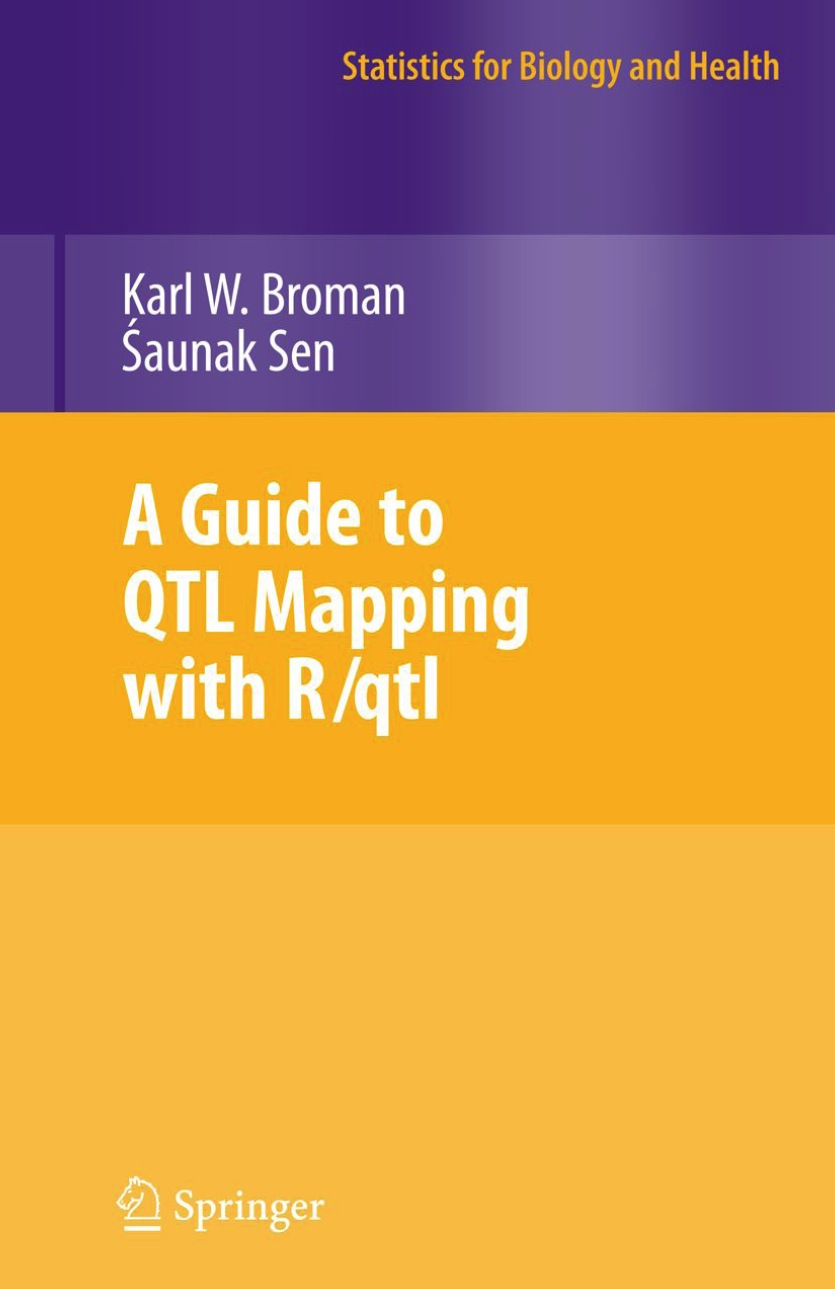
\includegraphics[height=6in]{Figs/book_cover_lg.jpg}}

\vfill

\smallestsize \color{mywhite} \verb|http://www.rqtl.org/book|


\newpage

\addtocounter{page}{-1}

\headsize \color{myyellow}
\hfill \begin{minipage}{5.75in}
\centering
Example
\end{minipage}

\vspace{30mm}

\hfill
\begin{minipage}{10in}
\smallersize \color{mywhite}
Sugiyama et al. Genomics 71:70-77, 2001

\vspace{16pt}

\smallestsize
\color{myblue}
250 male mice from the backcross (A $\times$ B) $\times$ B

Blood pressure after two weeks drinking water with 1\% NaCl
\end{minipage}

\vspace{15mm}


\centerline{\includegraphics{Figs/pheno.pdf}}

\newpage

\headsize \color{myyellow}
\hfill \begin{minipage}{5.75in}
\centering
Genetic map
\end{minipage}

\vfill

\centerline{\includegraphics{Figs/geneticmap.pdf}}


\newpage

\headsize \color{myyellow}
\hfill \begin{minipage}{5.75in}
\centering
Genotype data
\end{minipage}

\vfill

\centerline{\includegraphics{Figs/genodata.pdf}}


\newpage

\headsize \color{myyellow}
\hfill \begin{minipage}{5.75in}
\centering
Goals
\end{minipage}

\vspace{3cm}

\color{mywhite} \smallsize

\hfill \begin{minipage}[t]{9.5in}
\begin{itemize}
\itemsep24pt
\item Identify quantitative trait loci (QTL) \\[6pt]
   {\color{myblue}   (and interactions among QTL)}
\item Interval estimates of QTL location
\item Estimated QTL effects 
\end{itemize} \end{minipage}

\newpage

\headsize \color{myyellow}
\hfill \begin{minipage}{5.75in}
\centering
LOD curves
\end{minipage}

\vfill

\centerline{\includegraphics{Figs/alod2.pdf}}

\newpage

\headsize \color{myyellow}
\hfill \begin{minipage}{5.75in}
\centering
Estimated effects
\end{minipage}

\vfill

\centerline{\includegraphics{Figs/meffects.pdf}}

\newpage

\headsize \color{myyellow}
\hfill \begin{minipage}{5.75in}
\centering
Modeling multiple QTL 
\end{minipage}

\vspace{3cm}

\color{mywhite} \smallsize

\hfill \begin{minipage}[t]{10in}
\begin{itemize}
\itemsep24pt
\item Reduce residual variation $\longrightarrow$ increased power
   
\item Separate linked QTL

\item Identify interactions among QTL {\color{myblue} (epistasis)}

\end{itemize}
\end{minipage}


\newpage

\headsize \color{myyellow}
\hfill \begin{minipage}{5.75in}
\centering
Epistasis in BC
\end{minipage}

\vfill

\centerline{\includegraphics{Figs/epistasis_bc.pdf}}


\newpage

\headsize \color{myyellow}
\hfill \begin{minipage}{5.75in}
\centering
Epistasis in F$_{\mathsf{2}}$
\end{minipage}

\vfill

\centerline{\includegraphics{Figs/epistasis_f2.pdf}}



\newpage

\headsize \color{myyellow}
\hfill \begin{minipage}{5.75in}
\centering
2-dim, 2-QTL scan 
\end{minipage}

\vspace{2cm}

\color{mywhite} \smallsize

\hfill \begin{minipage}[t]{10in}
For all pairs of positions, fit the following models:

\vspace{10mm}

\hfill
\begin{minipage}{9in}
{\color{myblue}
$\mathsf{\text{H}_f: y = \mu + \beta_1 q_1 + \beta_2 q_2 +
      \gamma q_1 q_2 + \epsilon}$

\vspace{5mm}

$\mathsf{\text{H}_a: y = \mu + \beta_1 q_1 + \beta_2 q_2 +
      + \epsilon}$

\vspace{5mm}

$\mathsf{\text{H}_1: y = \mu + \beta_1 q_1 + \epsilon}$

\vspace{5mm}

$\mathsf{\text{H}_0: y = \mu + \epsilon}$

}
\end{minipage}

\vspace{20mm}

log$_{\mathsf{10}}$ likelihoods:

\vspace{5mm}

\hfill
\begin{minipage}{9in}
{\color{myblue}

$\mathsf{l_f(s,t)}$ \hspace{2cm}
$\mathsf{l_a(s,t)}$ \hspace{2cm}
$\mathsf{l_1(s)}$ \hspace{2cm}
$\mathsf{l_0}$ \hspace{2cm}
}
\end{minipage}


\end{minipage}


\newpage

\headsize \color{myyellow}
\hfill \begin{minipage}{5.75in}
\centering
2-dim, 2-QTL scan 
\end{minipage}

\vspace{2cm}

\color{mywhite} \smallsize

\hfill \begin{minipage}[t]{10in}
LOD scores:

\vspace{5mm}

\hspace{1cm}
\begin{minipage}{5in}
{\color{myblue}
\begin{eqnarray*}
\mathsf{\lod_f(s,t)}& = &\mathsf{l_f(s,t) - l_0} \\[24pt]
\mathsf{\lod_a(s,t)}& = &\mathsf{l_a(s,t) - l_0} \\[24pt]
\mathsf{\lod_i(s,t)}& = &\mathsf{l_f(s,t) - l_a(s,t)} \\[24pt]
\mathsf{\lod_1(s)}&   = &\mathsf{l_1(s) - l_0} \\[24pt]
\end{eqnarray*}
}
\end{minipage}



\end{minipage}


\newpage

\headsize \color{myyellow}
\hfill \begin{minipage}{5.75in}
\centering
Results: $\mathsf{\lod_i}$ and $\mathsf{\lod_f}$
\end{minipage}

\vfill 

\centerline{\includegraphics{Figs/2dscan_allchr.pdf}}

\newpage

\headsize \color{myyellow}
\hfill \begin{minipage}{5.75in}
\centering
Results: $\mathsf{\lod_i}$ and $\mathsf{\lod_f}$
\end{minipage}

\vfill 

\centerline{\includegraphics{Figs/2dscan_selchr.pdf}}

\newpage

\headsize \color{myyellow}
\hfill \begin{minipage}{5.75in}
\centering
Summaries
\end{minipage}

\vspace{15mm}

\color{mywhite} \smallsize

\hfill \begin{minipage}[t]{10in}
Consider each pair of chromosomes, {\color{myblue} $\mathsf{(j, k)}$}, \\
and let {\color{myblue} $\mathsf{c(s)}$} denote the chromosome for
  position {\color{myblue} $\mathsf{s}$}.

\vspace{5mm}

\hspace{1in}
\begin{minipage}{6in}
{\color{myblue}
\begin{eqnarray*}
\mathsf{\M_f(j,k)}& = &\mathsf{ \max_{c(s)=j, c(t)=k} \lod_f(s,t)} \\[12pt]
\mathsf{\M_a(j,k)}& = &\mathsf{ \max_{c(s)=j, c(t)=k} \lod_a(s,t)} \\[12pt]
\mathsf{\M_1(j,k)}& = &\mathsf{ \max_{c(s)=j \text{ or } k} \lod_1(s)} \\[36pt]
\mathsf{\M_i(j,k)}& = &\mathsf{ \M_f(j,k) - \M_a(j,k)}\\[12pt]
\mathsf{\M_{fv1}(j,k)}& = &\mathsf{ \M_f(j,k) - \M_1(j,k)}\\[12pt]
\mathsf{\M_{av1}(j,k)}& = &\mathsf{ \M_a(j,k) - \M_1(j,k)}
\end{eqnarray*}
}
\end{minipage}
\end{minipage}

\newpage

\headsize \color{myyellow}
\hfill \begin{minipage}{5.75in}
\centering
Results: $\mathsf{\lod_i}$ and $\mathsf{\lod_{fv1}}$
\end{minipage}

\vfill 

\centerline{\includegraphics{Figs/2dscan_selchr_fv1.pdf}}



\newpage

\headsize \color{myyellow}
\hfill \begin{minipage}{5.75in}
\centering
Thresholds
\end{minipage}

\vspace{20mm}

\color{mywhite} \smallersize

\hfill \begin{minipage}[t]{9.5in}
A pair of chromosomes {\color{myblue} $\mathsf{(j,k)}$} is considered interesting if:

\vspace{25mm}

{\color{myblue}
\centerline{$ \mathsf{\M_f(j,k)} > \mathsf{ T_f }$ \hspace{5mm} {\color{mypink} and } 
\hspace{5mm} 
{\color{mypink} \{} $ \mathsf{\M_{fv1}(j,k)} > \mathsf{ T_{fv1} }$ 
{\color{mypink} or } 
$ \mathsf{\M_i(j,k)} > \mathsf{ T_i }$  {\color{mypink} \}}}

\vspace{36pt}

\centerline{\color{mypink} or } 

\vspace{36pt}

\centerline{$ \mathsf{\M_a(j,k)} > \mathsf{ T_a }$ \hspace{5mm} {\color{mypink} and } 
\hspace{5mm} 
$ \mathsf{\M_{av1}(j,k)} > \mathsf{ T_{av1} }$ }
}


\vspace{25mm}

where the thresholds {\color{myblue} $\mathsf{(T_f, T_{fv1}, T_i, T_a,
    T_{av1})}$} are determined by a permutation test with a 2d scan

\end{minipage} \hspace{0.5in}


\newpage

\headsize \color{myyellow}
\hfill \begin{minipage}{5.75in}
\centering
2d scan summary
\end{minipage}

\vspace{40mm}

\color{mywhite} \smallersize

\begin{verbatim}
                   pos1f pos2f lod.full lod.fv1 lod.int
            c1:c4   71.3  30.0    14.36    6.78    0.27
            c6:c15  55.0  20.5     6.91    4.95    2.92
            c1:c1   39.3  78.3     5.10    1.58    0.09


                   pos1a pos2a  lod.add lod.av1
            c1:c4   68.3  30.0    14.09    6.50
            c6:c15  24.0  22.5     3.99    2.03
            c1:c1   48.3  79.3     5.02    1.50
\end{verbatim}



\newpage

\headsize \color{myyellow}
\hfill \begin{minipage}{5.75in}
\centering
Estimated effects
\end{minipage}

\vfill

\centerline{\includegraphics{Figs/ieffects.pdf}}


\newpage

\headsize \color{myyellow}
\hfill \begin{minipage}{5.75in}
\centering
Chr 1: $\mathsf{\lod_i}$ and $\mathsf{\lod_{av1}}$
\end{minipage}

\vfill

\centerline{\includegraphics{Figs/2dscan_chr1.pdf}}


%\newpage
%
%\headsize \color{myyellow}
%\hfill \begin{minipage}{5.75in}
%\centering
%Summaries
%\end{minipage}
%
%\vspace{15mm}
%
%\color{mywhite} \smallestsize
%
%
%\setlength{\tabcolsep}{0.15in}
%\renewcommand{\arraystretch}{1.5}
%\begin{center} \begin{tabular}{cccccccccccc} \\ \hline
%  chr      & \hspace{5mm} & \multicolumn{2}{c}{positions} & $\mathsf{\lod_f}$ 
%& $\mathsf{\lod_{fv1}}$ & $\mathsf{\lod_i}$ & 
%\hspace{5mm} &  \multicolumn{2}{c}{positions} & $\mathsf{\lod_a}$ 
%& $\mathsf{\lod_{av1}}$ \\ \hline 
%1 $\times$ 4 & & 68 & 30 &  14.04  &  \color{myhotpink} 6.43 &  0.295  &  &  68 & 30 &
%13.74 &  \color{myhotpink} 6.14 \\
%6 $\times$ 15 && 62 & 18 &   7.89  &  \color{myhotpink} 5.96 & \color{myhotpink} 3.960  &  &  25 & 20 &
%3.93 &   2.00 \\ \hline
%\end{tabular} \end{center}



\newpage

\headsize \color{myyellow}
\hfill \begin{minipage}{5.75in}
\centering
Hypothesis testing?
\end{minipage}

\vspace{2cm}

\color{mywhite} \smallersize

\hfill \begin{minipage}[t]{10in}
\begin{itemize}
\itemsep20mm
\item In the past, QTL mapping has been regarded as a task of
  {\color{mypink} hypothesis testing}.

\vspace{10mm}

\hspace{15mm} {\color{myblue} Is this a QTL?}

\vspace{10mm}

Much of the focus has been on adjusting for test multiplicity.
   
\item It is better to view the problem as one of {\color{mypink} model
  selection}.

\vspace{10mm}

\hspace{15mm} {\color{myblue} What set of QTL are well supported?}

\hspace{15mm} {\color{myblue} Is there evidence for QTL-QTL
  interactions?}

\vspace{10mm}

{\color{mypink} Model} $\mathsf{=}$ a defined set of QTL and QTL-QTL interactions
\\
(and possibly covariates and QTL-covariate interactions).

\end{itemize}
\end{minipage}

\newpage

\headsize \color{myyellow}
\hfill \begin{minipage}{5.75in}
\centering
Model selection
\end{minipage}

\vspace{15mm} \color{mywhite} \smallersize

\hspace{0.5in}
\begin{minipage}[t]{4in}
\vspace*{0mm}

\begin{itemize}
\item Class of models
{\smallestsize \color{myblue} \begin{itemize}
\item Additive models
\item + pairwise interactions
\item + higher-order interactions
\item Regression trees
\end{itemize} }

\vspace{15mm}

\item Model fit
{\smallestsize \color{myblue} \begin{itemize}
\item Maximum likelihood
\item Haley-Knott regression
\item extended Haley-Knott
\item Multiple imputation
\item MCMC
\end{itemize} }

\end{itemize}

\end{minipage} \hspace{1in}
\begin{minipage}[t]{4in}
\vspace*{0mm}

\begin{itemize}
\item Model comparison
{\smallestsize \color{myblue} \begin{itemize}
\item Estimated prediction error
\item AIC, BIC, penalized likelihood
\item Bayes
{\color{mybgcolor}
\item }
\end{itemize} }

\vspace{15mm}


\item Model search
{\smallestsize \color{myblue} \begin{itemize}
\item Forward selection
\item Backward elimination
\item Stepwise selection
\item Randomized algorithms 
\end{itemize} }


\end{itemize}

\end{minipage} 


\newpage

\headsize \color{myyellow}
\hfill \begin{minipage}{5.75in}
\centering
Target
\end{minipage}

\vspace{2cm} \color{mywhite} \smallersize

\hfill \begin{minipage}{10in}
\begin{itemize}
\itemsep24pt
\item Selection of a model includes two types of errors:

{\smallestsize
\begin{quote} \begin{itemize}
\item Miss important terms (QTLs or interactions)
\item Include extraneous terms
\end{itemize} \end{quote}}

\item Unlike in hypothesis testing, we can make {\color{mypink} both errors} at
the same time.

\item {\color{myyellow} Identify as many correct terms as possible, while
{\color{mypink} controlling the rate of inclusion of extraneous terms}.}

%\item You {\color{mypink} can't know} the performance of your procedure with your
%data---you need to know the truth.
%
%\item You {\color{myyellow} can know}:
%
%\smallestsize 
%\begin{quote} \begin{itemize}
%\setlength{\rightskip}{0pt plus 1fil} % makes ragged right
%\item How a particular procedure performs in simulated cases
%\item How a procedure performs in simulated data close to what you've inferred
%\end{itemize} \end{quote}


\end{itemize}
\end{minipage}


\newpage

\headsize \color{myyellow}
\hfill \begin{minipage}{5.75in}
\centering
What is special here?
\end{minipage}

\vspace{3cm} \color{mywhite} \smallersize

\hfill \begin{minipage}{10in}
\begin{itemize}
\itemsep24pt

\item Goal: identify the major players

\item A continuum of ordinal-valued covariates (the genetic loci)

\item Association among the covariates 
{\color{myblue} \smallestsize
\begin{itemize}
\item Loci on different chromosomes are independent
\item Along chromosome, a very simple (and known) correlation
  structure
\end{itemize} }

\end{itemize}
\end{minipage}





\newpage

\headsize \color{myyellow}
\hfill \begin{minipage}{5.75in}
\centering
Exploratory methods
\end{minipage}

\vspace{3cm} \color{mywhite} \smallersize

\hfill
\begin{minipage}{10in}
\begin{itemize}
\itemsep36pt
\item Condition on a large-effect QTL


{\color{myblue} \smallestsize
\begin{itemize}
\item Reduce residual variation
\item Conditional LOD score: 

\vspace{1cm}

\hspace{1in} $ \displaystyle{\mathsf{\lod(q_2 \ | \ q_1) = \text{log}_{10}
    \left\{\frac{\text{Pr}(\text{data} \ | \ q_1, q_2)}{
    \text{Pr}(\text{data} \ | \ q_1)}\right\} }}$
\end{itemize} }

\item Piece together the putative QTL from the 1d and 2d scans

{\color{myblue} \smallestsize
\begin{itemize}
\item Omit loci that no longer look interesting (drop-one-at-a-time analysis)
\item Study potential interactions among the identified loci
\item Scan for additional loci (perhaps allowing interactions), conditional on these
\end{itemize} }

\end{itemize}
\end{minipage}





\newpage

\headsize \color{myyellow}
\hfill \begin{minipage}{5.75in}
\centering
Controlling for chr 4
\end{minipage}

\vfill

\centerline{\includegraphics{Figs/alod_c4.pdf}}





\newpage

\headsize \color{myyellow}
\hfill \begin{minipage}{5.75in}
\centering
Drop-one-QTL table
\end{minipage}


\vspace{40mm}

\color{mywhite} \smallersize

\begin{verbatim}
                                  df    LOD   %var
                1@68.3             1   6.30   11.0
                4@30.0             1  12.21   20.1
                6@61.0             2   7.93   13.6
                15@17.5            2   7.14   12.3
                6@61.0 : 15@17.5   1   5.68    9.9
\end{verbatim}




\newpage

\headsize \color{myyellow}
\hfill \begin{minipage}{5.75in}
\centering
Automation
\end{minipage}

\vspace{3cm} \color{mywhite} \smallersize

\hfill \begin{minipage}{10in}
\begin{itemize}
\itemsep24pt

\item Assistance to the masses

\item Understanding performance

\item Many phenotypes

\end{itemize}
\end{minipage}


\newpage


\headsize \color{myyellow}
\hfill \begin{minipage}{5.75in}
\centering
Additive QTL
\end{minipage}

\vspace{2cm} \color{mywhite} \smallersize

\hfill \begin{minipage}{10in}

Simple situation:

{\smallestsize
\color{myblue}
\begin{itemize}
\item Dense markers
\item Complete genotype data
\item No epistasis

\end{itemize} }

\vspace{2cm}

\centerline{
$\mathsf{y  = \mu + \sum \beta_j \, q_j + \epsilon}$ \hspace{1cm}
       {\color{mypink} which $\mathsf{\beta_j \ne 0}$?}
}

\vspace{2cm}

{\color{myyellow}
$\mathsf{ \plod(\gamma) = \lod(\gamma) -
    {\color{mypink} T} \, |\gamma| }$
}




\end{minipage}



\newpage

\addtocounter{page}{-1}

\headsize \color{myyellow}
\hfill \begin{minipage}{5.75in}
\centering
Additive QTL
\end{minipage}

\vspace{2cm} \color{mywhite} \smallersize

\hfill \begin{minipage}{10in}

Simple situation:

{\smallestsize
\color{myblue}
\begin{itemize}
\item Dense markers
\item Complete genotype data
\item No epistasis

\end{itemize} }

\vspace{2cm}

\centerline{
$\mathsf{y  = \mu + \sum \beta_j \, q_j + \epsilon}$ \hspace{1cm}
       {\color{mypink} which $\mathsf{\beta_j \ne 0}$?}
}

\vspace{2cm}

{\color{myyellow}
$\mathsf{ \plod(\gamma) = \lod(\gamma) -
    {\color{mypink} T} \, |\gamma| }$
}

\vspace{2cm}

\begin{minipage}[t]{1.4in}
\vspace*{0mm}

0 vs 1 QTL: 
\end{minipage}
\begin{minipage}[t]{6in}
\vspace*{0mm} 

\color{myblue}
$\mathsf{\plod(\emptyset) = 0}$ \\[16pt]
$\mathsf{\plod(\{\lambda\}) =
    \lod(\lambda) - {\color{mypink} T}}$ 
\end{minipage}


\end{minipage}



\newpage

\addtocounter{page}{-1}

\headsize \color{myyellow}
\hfill \begin{minipage}{5.75in}
\centering
Additive QTL
\end{minipage}

\vspace{2cm} \color{mywhite} \smallersize

\hfill \begin{minipage}{10in}

Simple situation:

{\smallestsize
\color{myblue}
\begin{itemize}
\item Dense markers
\item Complete genotype data
\item No epistasis

\end{itemize} }

\vspace{2cm}

\centerline{
$\mathsf{y  = \mu + \sum \beta_j \, q_j + \epsilon}$ \hspace{1cm}
       {\color{mypink} which $\mathsf{\beta_j \ne 0}$?}
}

\vspace{2cm}

{\color{myyellow}
$\mathsf{ \plod(\gamma) = \lod(\gamma) -
    {\color{mypink} T} \, |\gamma| }$
}

\vspace{2cm}

\begin{minipage}[t]{10in}
\vspace*{0mm}

For the mouse genome: \\[6pt]
\hspace*{0.5in} $\mathsf{\color{mypink} T}$ = {\color{myblue}
  2.69} (BC) or {\color{myblue} 3.52} (F$_{\mathsf{2}}$)
\end{minipage}

\end{minipage}




\newpage

\headsize \color{myyellow}
\hfill \begin{minipage}{5.75in}
\centering
Experience
\end{minipage}

\vspace{3cm} \color{mywhite} \smallersize

\hfill \begin{minipage}{10in}

\begin{itemize}
\itemsep18pt
\item Controls rate of inclusion of extraneous terms
\item Forward selection over-selects
\item {\color{myblue} Forward selection followed by backward elimination} works as well
  as {\color{myblue} MCMC}

\item {\color{mypink} Need to define performance criteria}
\item {\color{mypink} Need large-scale simulations}
\end{itemize}

\vspace{6cm}

\smallestsize \color{myblue}
\hfill Broman \& Speed, JRSS B 64:641-656, 2002

\end{minipage}


\newpage

\headsize \color{myyellow}
\hfill \begin{minipage}{5.75in}
\centering
Epistasis
\end{minipage}

\vspace{3cm} \color{mywhite} \smallersize

\hfill \begin{minipage}{10in}

\centerline{
$\mathsf{y  = \mu + \sum \beta_j \, q_j + \sum \gamma_{jk} \, q_j \,
    q_k + \epsilon}$
}

\vspace{3cm}

{\color{myyellow}
$\mathsf{ \plod(\gamma) = \lod(\gamma) -
    {\color{mypink} T_m} \, |\gamma|_m - {\color{mypink} T_i} \, |\gamma|_i }$
}


\vspace{15mm}

\hspace{3cm} $\mathsf{\color{mypink} T_m}$ = as chosen previously

\vspace{15mm}

\hspace{3cm} $\mathsf{\color{mypink} T_i}$ = ?



\end{minipage}



\newpage

\headsize \color{myyellow}
\hfill \begin{minipage}{5.75in}
\centering
Idea 1
\end{minipage}

\vspace{3cm} \color{mywhite} \smallersize

\hfill \begin{minipage}{10in}

Imagine there are two additive QTL and consider a 2d, 2-QTL scan.

\vspace{1cm}

\hspace*{0.5in} $\mathsf{\color{mypink} T_i}$ = 95th percentile of the
  distribution of \\[6pt]
\hspace*{1.3in} {\color{myblue} $\mathsf{ \text{max} \, \lod_f(s,t) -
    \text{max} \, \lod_a(s,t)}$}


\end{minipage}



\newpage

\addtocounter{page}{-1}

\headsize \color{myyellow}
\hfill \begin{minipage}{5.75in}
\centering
Idea 1
\end{minipage}

\vspace{3cm} \color{mywhite} \smallersize

\hfill \begin{minipage}{10in}

Imagine there are two additive QTL and consider a 2d, 2-QTL scan.

\vspace{1cm}

\hspace*{0.5in} $\mathsf{\color{mypink} T_i}$ = 95th percentile of the
  distribution of \\[6pt]
\hspace*{1.3in} {\color{myblue} $\mathsf{ \text{max} \, \lod_f(s,t) -
    \text{max} \, \lod_a(s,t)}$}


\vspace{2cm}

For the mouse genome: \\[12pt]
\hspace*{0.5in} $\mathsf{\color{mypink} T_m}$ = {\color{myblue}
  2.69} (BC) or {\color{myblue} 3.52} (F$_{\mathsf{2}}$) \\[12pt]
\hspace*{0.5in} $\mathsf{\color{mypink} T^H_i}$ = {\color{myblue}
  2.62} (BC) or {\color{myblue} 4.28} (F$_{\mathsf{2}}$)


\end{minipage}



\newpage

\headsize \color{myyellow}
\hfill \begin{minipage}{5.75in}
\centering
Idea 2
\end{minipage}

\vspace{3cm} \color{mywhite} \smallersize

\hfill \begin{minipage}{10in}

Imagine there is one QTL and consider a 2d, 2-QTL scan.

\vspace{1cm}

\hspace*{0.5in} $\mathsf{\color{mypink} T_m + T_i}$ = 95th percentile of the
  distribution of \\[6pt]
\hspace*{2.0in} {\color{myblue} $\mathsf{ \text{max} \, \lod_f(s,t) -
    \text{max} \, \lod_1(s)}$}


\end{minipage}



\newpage

\addtocounter{page}{-1}

\headsize \color{myyellow}
\hfill \begin{minipage}{5.75in}
\centering
Idea 2
\end{minipage}

\vspace{3cm} \color{mywhite} \smallersize

\hfill \begin{minipage}{10in}

Imagine there is one QTL and consider a 2d, 2-QTL scan.

\vspace{1cm}

\hspace*{0.5in} $\mathsf{\color{mypink} T_m + T_i}$ = 95th percentile of the
  distribution of \\[6pt]
\hspace*{2.0in} {\color{myblue} $\mathsf{ \text{max} \, \lod_f(s,t) -
    \text{max} \, \lod_1(s)}$}


\vspace{2cm}

For the mouse genome: \\[12pt]
\hspace*{0.5in} $\mathsf{\color{mypink} T_m}$ = {\color{myblue}
  2.69} (BC) or {\color{myblue} 3.52} (F$_{\mathsf{2}}$) \\[12pt]
\hspace*{0.5in} $\mathsf{\color{mypink} T^H_i}$ = {\color{myblue}
  2.62} (BC) or {\color{myblue} 4.28} (F$_{\mathsf{2}}$) \\[12pt]
\hspace*{0.5in} $\mathsf{\color{mypink} T^L_i}$ = {\color{myblue}
  1.19} (BC) or {\color{myblue} 2.69} (F$_{\mathsf{2}}$)


\end{minipage}









\newpage

\headsize \color{myyellow}
\hfill \begin{minipage}{5.75in}
\centering
Models as graphs
\end{minipage}

\vfill

\centerline{\includegraphics{Figs/models.pdf}}







\newpage

\headsize \color{myyellow}
\hfill \begin{minipage}{5.75in}
\centering
Results
\end{minipage}

\vfill


\centerline{\includegraphics{Figs/hyper_models1.pdf}}



\newpage

\addtocounter{page}{-1}

\headsize \color{myyellow}
\hfill \begin{minipage}{5.75in}
\centering
Results
\end{minipage}

\vfill


\centerline{\includegraphics{Figs/hyper_models2.pdf}}



\newpage

\addtocounter{page}{-1}

\headsize \color{myyellow}
\hfill \begin{minipage}{5.75in}
\centering
Results
\end{minipage}

\vfill


\centerline{\includegraphics{Figs/hyper_models3.pdf}}


\newpage

\headsize \color{myyellow}
\hfill \begin{minipage}{5.75in}
\centering
Profile LOD curves
\end{minipage}

\vfill


\centerline{\includegraphics{Figs/lod_profile.pdf}}


\newpage

\headsize \color{myyellow}
\hfill \begin{minipage}{5.75in}
\centering
Drop-one-QTL table
\end{minipage}


\vspace{40mm}

\color{mywhite} \smallersize

\begin{verbatim}
                                  df    LOD   %var
                1@68.3             1   6.30   11.0
                4@30.0             1  12.21   20.1
                6@61.0             2   7.93   13.6
                15@17.5            2   7.14   12.3
                6@61.0 : 15@17.5   1   5.68    9.9
\end{verbatim}

\newpage


\headsize \color{myyellow}
\hfill \begin{minipage}{5.75in}
\centering
Add an interaction?
\end{minipage}

\vfill


\centerline{\includegraphics{Figs/hyper_models4.pdf}}



\newpage

\addtocounter{page}{-1}

\headsize \color{myyellow}
\hfill \begin{minipage}{5.75in}
\centering
Add an interaction?
\end{minipage}

\vfill


\centerline{\includegraphics{Figs/hyper_models5.pdf}}



\newpage

\addtocounter{page}{-1}

\headsize \color{myyellow}
\hfill \begin{minipage}{5.75in}
\centering
Add an interaction?
\end{minipage}

\vfill


\centerline{\includegraphics{Figs/hyper_models6.pdf}}



\newpage

\addtocounter{page}{-1}

\headsize \color{myyellow}
\hfill \begin{minipage}{5.75in}
\centering
Add an interaction?
\end{minipage}

\vfill


\centerline{\includegraphics{Figs/hyper_models7.pdf}}



\newpage

\addtocounter{page}{-1}

\headsize \color{myyellow}
\hfill \begin{minipage}{5.75in}
\centering
Add an interaction?
\end{minipage}

\vfill


\centerline{\includegraphics{Figs/hyper_models8.pdf}}




\newpage


\headsize \color{myyellow}
\hfill \begin{minipage}{5.75in}
\centering
Add another QTL?
\end{minipage}

\vfill


\centerline{\includegraphics{Figs/hyper_models9.pdf}}



\newpage


\addtocounter{page}{-1}

\headsize \color{myyellow}
\hfill \begin{minipage}{5.75in}
\centering
Add another QTL?
\end{minipage}

\vfill


\centerline{\includegraphics{Figs/hyper_models10.pdf}}



\newpage


\addtocounter{page}{-1}

\headsize \color{myyellow}
\hfill \begin{minipage}{5.75in}
\centering
Add another QTL?
\end{minipage}

\vfill


\centerline{\includegraphics{Figs/hyper_models11.pdf}}



\newpage



\headsize \color{myyellow}
\hfill \begin{minipage}{5.75in}
\centering
Add a pair of QTL?
\end{minipage}

\vfill


\centerline{\includegraphics{Figs/hyper_models12.pdf}}






%\newpage
%
%\headsize \color{myyellow}
%\hfill \begin{minipage}{5.75in}
%\centering
%To do
%\end{minipage}
%
%\vspace{3cm} \color{mywhite} \smallersize
%
%\hfill \begin{minipage}{10in}
%
%\begin{itemize}
%\itemsep18pt
%\item Improve search procedures
%\item Measuring model uncertainty
%\item Measuring uncertainty in QTL location
%\end{itemize}
%
%\end{minipage}





\newpage

\headsize \color{myyellow}
\hfill \begin{minipage}{5.75in}
\centering
Summary
\end{minipage}

\vspace{3cm} \color{mywhite} \smallersize

\hfill \begin{minipage}{9.5in}

\begin{itemize}
\itemsep24pt
\item QTL mapping is a model selection problem
\item The criterion for comparing models is most important
\item We're focusing on a penalized likelihood method, with penalties
  derived from permutation tests with 1d and 2d scans
\item Manichaikul et al., Genetics 181:1077--1086, 2009
\end{itemize}

\end{minipage} \hspace{0.5in}



\end{document}
